\chapter{Results}
\label{chap:results}
The results in the scientific section will be in relation to the research question and hypothesis. The engineering section will present how many product goals were achieved at time of delivery. The final section shows all of the administrative results. Including project planning, time sheets and documentation of our development process.

\section{Scientific Results}
% TODO first two sentences
The management \acrshort{API} and deployment trigger may be protected from the internet in a self-hosted solution. By potentially operating on a physically separated network when this would be impractical or impossible in an external solution. It was found that in an external solution, it is necessary to trust the host with credentials giving them access to the environment \acrshort{API}s.


The following table describes the count of each attack class in the hypothetical external solution and self-hosted solution, where $n$ is the number of environments managed by the \acrshort{CD} solution:
\begin{table}[ht]
    \begin{tabularx}{\textwidth}{|X|c|c|}
        \hline
        \textbf{Attack class}                  & \textbf{External} & \textbf{Self-hosted}\\ \hline \hline
        open\_TCP/UDP-socket                   & 0 & 0        \\ \hline
        open\_TCP/UDP-socket                   & $1+n$ & $1+n$\\ \hline
        world-accessible\_TCP/UDP-socket       & $1+n$ & 0    \\ \hline
        open\_unsecured\_env-mgmt              & 0     & 0    \\ \hline
        open\_secured\_env-mgmt                & 0     & n    \\ \hline
        world\_accessible\_secured\_env-mgmt   & n     & 0    \\ \hline
        third-party\_credentials               & n     & 0    \\ \hline
        world-accessible\_deployment-trigger   & 1     & 0    \\ \hline
        locally-accessible\_deployment-trigger & 1     & 1    \\ \hline
    \end{tabularx}
    \caption{The number of times each attack class appears in the solutions}
    \label{tab:result1}
\end{table}

Table \ref{tab:result1} describes the weighted sum, estimating the attack surface, of the hypothetical external solution and self-hosted solution:
\begin{table}[ht]
    \begin{tabularx}{\textwidth}{|X|c|c|}
        \hline
        \textbf{Solution}  & \textbf{Attack surface} & \textbf{Sum}\\ \hline \hline
        External           & $0.3\times(1+n) + 0.4\times(1+n) + 0.3\times n + n + 0.6 + 0.4$ & $2n + 1.7$\\ \hline
        Self-hosted        & $0.3\times(1+n) + 0.2\times(n) + 0.4$ & $(n + 1.4)/2$\\ \hline
    \end{tabularx}
    \caption{The attack surfaces of the solutions}
    \label{tab:result1}
\end{table}

\begin{center}
    \begin{figure}
        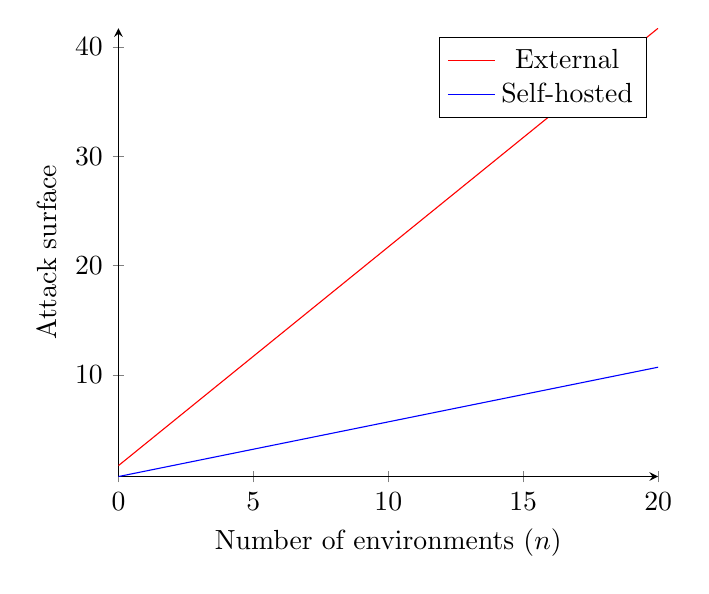
\begin{tikzpicture}
        \begin{axis}[
            axis lines = left,
            xlabel = {Number of environments ($n$)},
            ylabel = {Attack surface},
        ]
        %Below the red parabola is defined
        \addplot [
            domain=0:20, 
            samples=100, 
            color=red,
        ]
        {2*x + 1.7};
        \addlegendentry{External}
        %Here the blue parabloa is defined
        \addplot [
            domain=0:20, 
            samples=100, 
            color=blue,
            ]
            {0.5*x + 0.7};
        \addlegendentry{Self-hosted}
        \end{axis}
        \end{tikzpicture}
        \caption{Attack surface graph}
        \label{fig:my_label}
    \end{figure}
\end{center}

\section{Engineering Results}
\label{subsec:engineering}
\subsection{Security}
Throughout the development of cion the authors have learned how to securely implement a \acrshort{CD} solution. There are 2 key areas of an \acrshort{CD} system that needs to be secure: (1) the deployment trigger, and (2) the environment management \acrshort{API}.

Securing (1) is important so that somebody who does not have explicit permission to alter the environments can start or stop running services. If an external deployment trigger does not verify the permissions, an attacker could easily perform a \textit{denial-of-service} attack against any service in the environment.

An ideal security solution would implement a \acrfull{CA} where certificates can be issued and retracted. However a priority for cion was to support external triggers from DockerHub, unfortunately DockerHub does not allow custom webhooks. As such it was impossible to implement a \acrshort{CA} and support DockerHub. Since the only customiseable part of the DockerHub webhook is the \acrshort{URL} we settled on making the \textit{deployment trigger} \acrshort{URL} path a secret. This means that an attacker would have to figure out the \acrshort{URL} of the \textit{deployment trigger} to exploit the system. 

(2) is more security sensitive than (1), if an attacker gains access to an environment's management \acrshort{API} they essentially gain admininistrator access to the environment's servers. As such container orchestrators like Docker Swarm and Kubernetes support authorisation through a \acrfull{TLS} certificate. The authors wanted cion to support multiple connection modes to container orchestrators, three connection modes are supported:

\begin{itemize}
    \item \textbf{Docker socket}(insecure): Docker Swarm supports management through a unix socket. Docker socket does not secure this socket and as such it should not be used outside of local development. 
    \item \textbf{Docker TLS}: Docker does support TLS authorisation, although the administrators have to create the certificates themselves with an error prone method described in out system documentation. When configured properly it is secure, but care should be taken when creating the certificates. 
    \item \textbf{Kubernetes Service accounts}: Kubernetes supports authorisation through service accounts. These service accounts are easy to setup and in the background they also use \acrshort{TLS} for authentication.
\end{itemize}

All of the secrets managed by cion are stored outside the database in the docker secrets system.

\subsection{Code Refactoring}
\label{sec:coderefactoring}
A substantial amount of time was spent refactoring code from the autumn project. This was to make the codebase more consistent, fix bugs and improve performance. One of the major changes was going from PyRX to aioreactive. The other major change was converting from flask to aiohttp in the catalyst component. 


% Planned features where implemented

% The feature implementation to add support for cion to deploy to Kubernetes turned out to be pretty simple compared to docker. This due to how Kubernetes requires

\subsection{Implemented Features}
The following chapters cover if and how the features defined by the User Profiles in the vision document, appendix \ref{appendix:vision}, were implemented. There are two additional chapters describing features that were not yet planned at this stage, but these are minor in comparison to the ones defined by the user profiles, and mostly focus on increasing ease of use in the web \acrshort{ui}.

\subsubsection{Kubernetes Support}
Kubernetes support was a highly regarded feature and was implemented as specified in the requirements document. Cion now has the ability to manage services in Kubernetes environments.

Configuring cion to manage a Kubernetes environment is done the same way as a Docker environment.


\subsubsection{Webhooks (Post-Deploy Behaviour)}
A new page that has been added to the web UI is the Webhooks page. It is used to configure the new webhook-feature. This feature allows the user to configure webhooks to trigger on specific events within the cion solution, for example when cion receives a new image or when a service is updated. 

Webhooks are highly configurable, but this comes at the cost of them being complicated to configure, and requires a low-level understanding of the cion solution if the user wants to do something complicated. This is explained thoroughly in the end-user documentation. The complete list of configuration-options for the webhooks-feature is:

\begin{itemize}
    \item URL
    \item Headers
    \item Event
    \item Filters/triggers
    \item Body
\end{itemize}

The \textbf{URL} is the URL the webhook will send the \textit{POST}-request to.

The \textbf{headers} are what HTTP-headers send to the \textbf{URL}.

The \textbf{event}-field is a select-box. The user has to select one of the options provided, for example \textit{service-update}. 
When an event of the type selected occurs cion will run the events data through all the configured \textbf{filters}. The filters are regex-patterns that all have to match for the webhook to be fired. A filter is configured with a name and a value. The name is the name of the field in the event data, and the value is the regex-pattern that has to match that data for the filter to pass.

The \textbf{body} is the body of the HTTP-request that is sent to the configured\textbf{URL}. It supports the python format-function. As such the user can insert fields from the event data into the body by using curly brackets around field-names in the text. For example:

\begin{verbatim}
    {{
        "service-name": "{service}"
    }}
\end{verbatim}

The above example generates a JSON-body containing exactly one key-value-pair, containing the service-name extracted from the event data. 
The user has to escape curly brackets, as shown above, due to how python's format-function tries to interpret them as variable-names.
The above body-string would result in the following when the field "service" in the event data is "cion\_api":

\begin{verbatim}
    {
        "service-name": "cion_api"
    }
\end{verbatim}

This example used JSON as the content type, but any string and formatting is supported. 


\subsubsection{Permissions}
A permissions system was implemented to allow administrators to specify what features of cion a user should have access to. The administrator can permit or deny access to service configuration on specific environments, environment configuration and cion-features like user-administration and log- and configuration-viewing.


\subsubsection{Service Update Scheduling (Scheduled Deployment)}
The individual service page has gotten an upgrade and a new feature was added; service update scheduling. It allows users to schedule updates to services to specific times and dates.


\subsubsection{Environments}
A new page was added where the user can configure and add environments for their cion instance to manage. It supports adding Kubernetes environments, and docker environments over TLS or the docker socket.


\subsubsection{User Settings/Profile Page}
The \textit{user settings}-, now named the \textit{profile}-page is implemented as specified in the requirements document. With fields to change the logged in user's password and gravatar-email. The user will only be able to change the password if they enter their old password. After changing their password they are logged out.


\subsection{User-Test}
Towards the end of the development period a test with an intended end user was conducted. Questions and the subject's answers are listed in appendix \ref{appendix:usertest}.

The test was productive in uncovering bugs and bad implementations considering \acrfull{ux}. The test-subject was overall pleased with the product, but noted that some of the bugs they uncovered needed to be patched before they could use it for their production environment. The bugs reported were fixed shortly after completing the test.


\section{Administrative Results}
\subsection{Goal Achievement}
There were multiple deviations from the original project plan. Partly because some parts were overestimated, and others were underestimated. The mandatory work in February was also not considered in the first project plan, which meant some features were pushed down the line. The biggest deviations were for Kubernetes support and scheduled deployment. In which the hours needed to integrate Kubernetes support were severly underestimated, but this was partly balanced out by overestimating the hours needed to implement scheduled deployment. Kubernetes support was planned for finalisation by the end of March, but ended up being finished in late April. Meanwhile scheduled delivery was due in the middle of April but was already done at the start of March. Exact deviations in hours can be found in the timesheet in appendix \ref{appendix:projecthandbook}.


\subsection{Process}
%Discuss how we went about development
The team's development process was a mixture of several different agile methods with tweaks and adjustments. We used parts of SCRUM. We skipped daily stand-up meetings, but we did have weekly meetings with the product owner. We used a SCRUM-board on Atlassian's Jira to manage and track tasks. As a rule of thumb the team decided to do most of the work between 10.00-15.00 from Monday through Friday. The concept of sprints was also a part of SCRUM we dropped. Even though we did not use sprints, we did work in an iterative manner. Every meeting with the product owner gave us more feedback that either changed or created tasks on our SCRUM-board.

\begin{figure}[h!]
  \includegraphics[width=\linewidth,height=\textheight,keepaspectratio]{images/scrum_board.png}
  \caption{Scrum board}
  \label{fig:scrumboard}
\end{figure}


\begin{figure}[h!]
  \includegraphics[width=\linewidth,height=\textheight,keepaspectratio]{images/task_list.png}
  \caption{Task list}
  \label{fig:tasklist}
\end{figure}

\subsection{Documentation}
Most of the documentation for cion is written in markdown\cite{github-markdown} formatting. This allows it to be hosted on sites like github.com and readthedocs.io. Hosting on github makes the documentation accessible for the target users for cion, which are developers and system administrators. Github is a development platform to host and review code and manage projects\cite{github}.
